\section{Introduction}
Computer processors are now capable of running hundreds of threads of execution simultaneously in parallel. With severe physical limits on clock speed, future architectures will likely support more simultaneous threads rather than faster individual cores ~\cite{intropaper}. These advances provides programmers new way to speed up their programs. However, simply using more threads to exexute parts of the program does not guarantee speedup and may very well speed down than speed up. In fact, it is not uncommon for a program’s overall throughput to decrease when thread count grows large enough ~\cite{intropaper}. So, to speedup genomics software with multiple number of threads, programmers should deliberate on how they should structure the entire program and how many threads they should use so that the overhead of multithreading will not outweigh the speedup it brings.

Here we try to solve the problem of decompressing a gzip compressed FASTQ files in parallel by building indices over it. 
This startegies of building indices can scale to hundreds of threads and make it easier for our program to be part of the pipeline of other multithreading or multiprocessing genomics tools. 
\subsection{Challenge of Multithreading}
Some of the challenges multithreading will pose can be seen in Figure 1. Figure 1 shows how bad multithreading can be if handled incorrectly. We can see that if a thread needs to read from or write to a file, it needs exclusive right to the file so that the file won't be changed when it's reading it. This is usually done by using locks. Unfortunately, even though multiple threads can have read lock of the same file, operating system does not really allows them to read the file simultaneously. That means if multiple thread is trying to read a file, most of them cannot do anything and has to wait for that one thread to complete first. The same applies to writing to a file as well. Therefore, it's important to structure the program and choose parameters wisely so that the time spent waiting for each thread is minimum. 
\begin{figure}[H]
    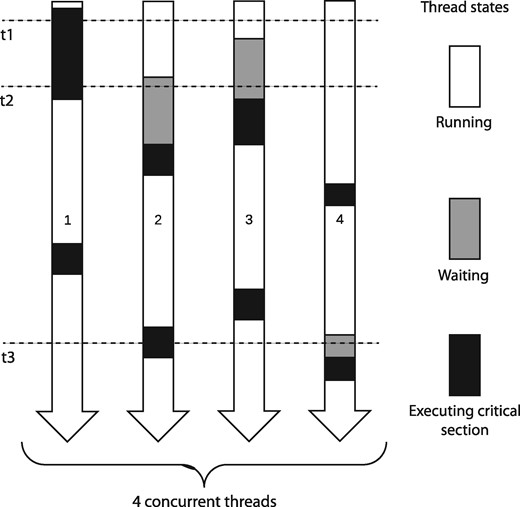
\includegraphics[width=\linewidth]{figs/multithread.jpeg}
    \label{fig:multithread}
    \caption{This figure shows 4 threads running simultaneously . Time progress from top to bottom. Gray area represents time spent waiting instead of operating. Black area represents threads doing operations that require exclusive rights to certain resources. ~\cite{intropaper}}
\end{figure}

